\section{Risultati e discussione}\label{sec:risultati}
In questa sezione verranno discussi e confrontati i risultati che i tre modelli nelle varie versioni hanno raggiunto nella fase di testing sul test set.

Dalla tabella \ref{tab:resdt} si nota che la versione migliore del Decision tree è la terza, quella in ensemble, infatti supera le prime due in tutte le metriche e raggiunge una precisione molto alta.

\begin{table}[h] 
\centering
\begin{tabular}{l l l l l}
\hline
\textbf{Versione} & \textbf{Accuracy bilanciata} & \textbf{Precision} & \textbf{Recall} & \textbf{F1-score}\\
\hline
Versione 1 & 0.976 & 0.986 & 0.986 & 0.986 \\
Versione 2 & 0.973 & 0.984 & 0.984 & 0.984 \\
\textbf{Versione 3} & \textbf{0.993} & \textbf{0.996} & \textbf{0.996} & \textbf{0.996} \\
\hline
\end{tabular}
\caption{Prestazioni delle varianti del Decision tree.}
\label{tab:resdt}
\end{table}

In tabella \ref{tab:ressvm} invece vediamo i risultati delle tre versioni del modello SVM, dai quali si deduce che anche in questo caso la versione migliore è quella in ensemble in quanto migliora di circa il 15-20\% i risultati delle prime due versioni, grazie proprio alla combinazione dei risultati di più modelli, cosiddetti weak learner, in un risultato unico. I risultati raggiunti comunque non sono soddisfacenti e non sono paragonabili a quelli che garantisce il Decision tree.

\begin{table}[h] 
\centering
\begin{tabular}{l l l l l}
\hline
\textbf{Versione} & \textbf{Accuracy bilanciata} & \textbf{Precision} & \textbf{Recall} & \textbf{F1-score}\\
\hline
Versione 1 & 0.420 & 0.551 & 0.490 & 0.482 \\
Versione 2 & 0.440 & 0.500 & 0.452 & 0.434 \\
\textbf{Versione 3} & \textbf{0.610} & \textbf{0.675} & \textbf{0.655 } & \textbf{0.620} \\
\hline
\end{tabular}
\caption{Prestazioni delle varianti dell'SVM.}
\label{tab:ressvm}
\end{table}

In tabella \ref{tab:resnn} sono confrontati i risultati della rete neurale nelle tre versioni, e come si vede la migliore è anche in questo caso la terza, anche se la differenza con la seconda versione è minima quindi l'incremento di prestazioni dato dall'ensemble è trascurabile in questo caso, seppur non nullo.

\begin{table}[h] 
\centering
\begin{tabular}{l l l l l}
\hline
\textbf{Versione} & \textbf{Accuracy bilanciata} & \textbf{Precision} & \textbf{Recall} & \textbf{F1-score}\\
\hline
Versione 1 & 0.963 & 0.981 & 0.981 & 0.981 \\
Versione 2 & 0.986 & 0.991 & 0.991 & 0.991 \\
\textbf{Versione 3} & \textbf{0.990} & \textbf{0.993} & \textbf{0.993} & \textbf{0.993} \\
\hline
\end{tabular}
\caption{Prestazioni delle varianti della rete neurale.}
\label{tab:resnn}
\end{table}

Infine in tabella \ref{tab:resbest} sono messi a confronto i tre modelli nelle loro versioni migliori, come si vede l'algoritmo che performa meglio è il Decision tree, anche se la rete neurale ha prestazioni molto simili, solo leggermente inferiori, invece la SVM ha prestazioni nettamente inferiori e quindi è sconsigliata in questo problema.

\begin{table}[h] 
\centering
\begin{tabular}{l l l l l}
\hline
\textbf{Modello} & \textbf{Accuracy bilanciata} & \textbf{Precision} & \textbf{Recall} & \textbf{F1-score}\\
\hline
\textbf{Decision Tree} & \textbf{0.993} & \textbf{0.996} & \textbf{0.996} & \textbf{0.996} \\
SVM & 0.610 & 0.675 & 0.655 & 0.620 \\
Rete neurale & 0.990 & 0.993 & 0.993 & 0.993 \\
\hline
\end{tabular}
\caption{Confronto tra le migliori versioni dei tre modelli analizzati.}
\label{tab:resbest}
\end{table}

In tutti e tre i modelli la versione migliore è risultata essere la terza, grazie all'incremento di prestazioni garantito dall'ensemble, nel caso però della SVM e della rete neurale questo avviene a un costo di efficienza in termini di velocità, infatti applicando il metodo Bagging il processo di training è rallentato considerevolmente rispetto alle prime due versioni. Questo rallentamento non avviene nel caso del Decision tree, infatti il RandomForest ha tempi paragonabili alla versione non in ensemble. 

In figura \ref{fig:conf} sono rappresentate le tre confusion matrix delle versioni migliori dei tre modelli, i valori sono normalizzati in questo caso, quindi non sono mostrati i valori assoluti ma la percentuale sul totale. Come si vede le matrici del Decision tree e della rete neurale hanno valori prossimi a uno sulla diagonale principale, il che significa che i valori predetti per una classe sono quasi tutti corretti. Al contrario la matrice del modello SVM ha valori minori nella diagonale principale, a dimostrazione del fatto che le prestazioni di questo algoritmo non sono eccellenti. 

\begin{figure}[h]
    \centering
    \begin{subfigure}[t]{0.4\textwidth}
        \centering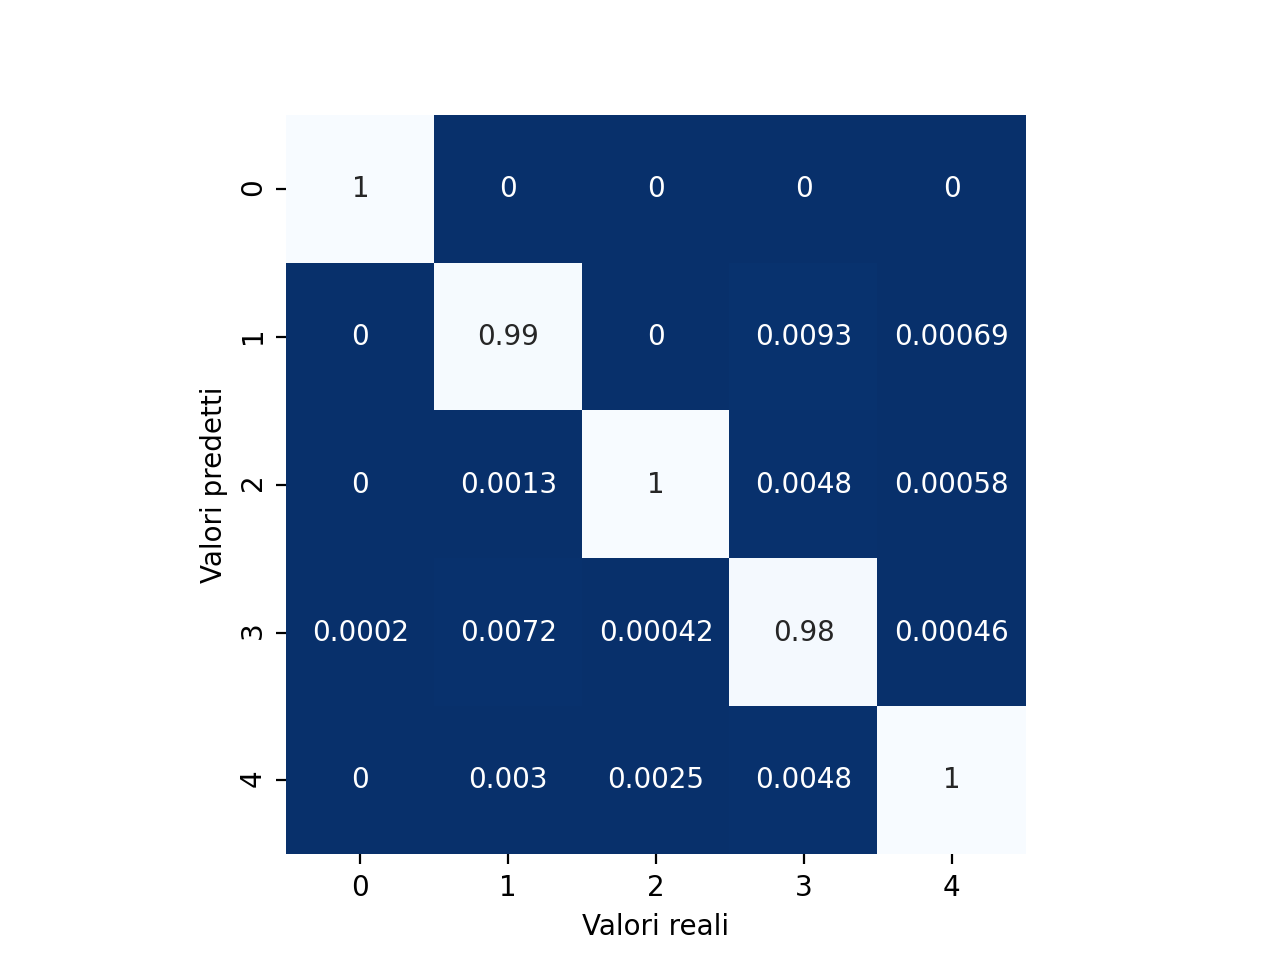
\includegraphics[width=1\linewidth]{confdt}
        \caption{Confusion matrix della terza versione del Decision tree.}
        \label{fig:conf:dt}
    \end{subfigure}
    %
    \begin{subfigure}[t]{0.4\textwidth}
        \centering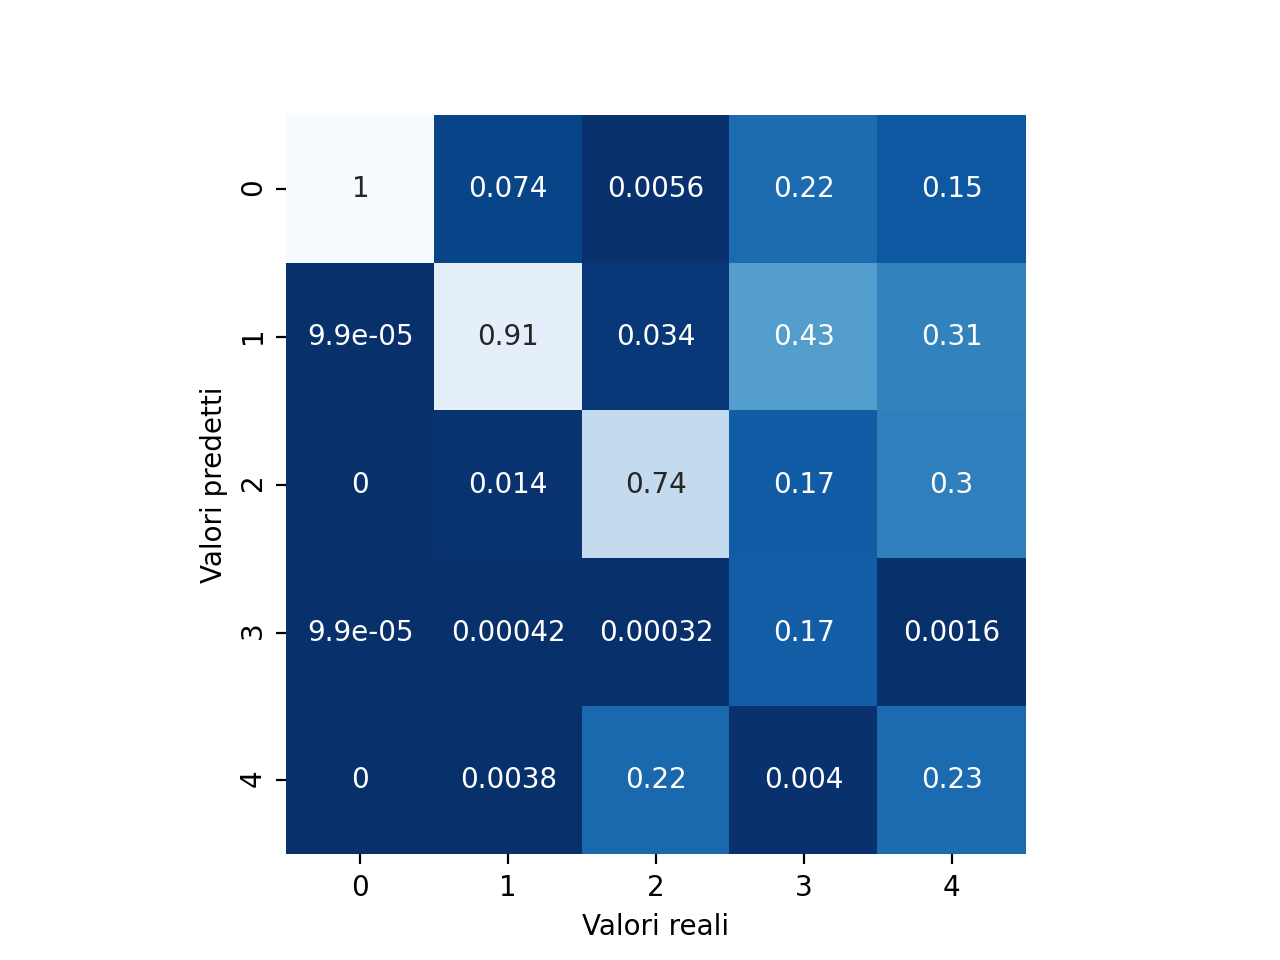
\includegraphics[width=1\linewidth]{confsvm}
        \caption{Confusion matrix della terza versione dell'SVM.}
        \label{fig:conf:svm}
    \end{subfigure}
    %
    \\
    \begin{subfigure}[t]{0.4\textwidth}
        \centering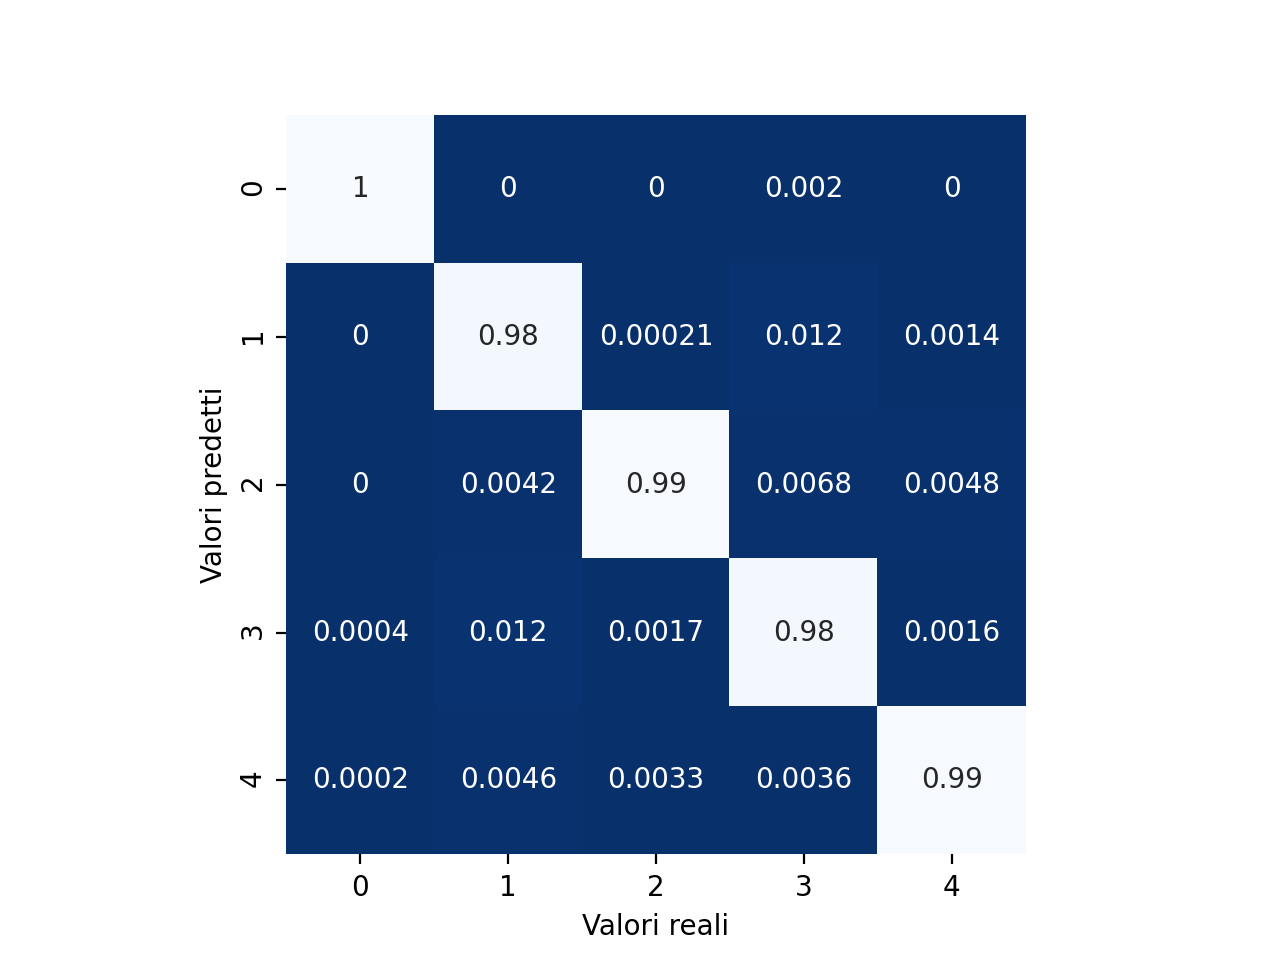
\includegraphics[width=1\linewidth]{confnn}
        \caption{Confusion matrix della terza versione della rete neurale.}
        \label{fig:conf:nn}
    \end{subfigure}
    %
    \caption{Confusion matrix dei tre modelli migliori.}
    \label{fig:conf}
\end{figure}

Per questo progetto sia la SVM che la rete neurale sono state testate con dei valori per gli iperparametri non ottimali, infatti per questioni di tempo e hardware a disposizione è stato deciso di non usare valori troppo alti per alcuni degli iperparametri, che probabilmente avrebbero portato a risultati migliori ma a discapito del tempo di training e di model selection, tenendo conto anche del fatto che il dataset usato contiene un notevole numero di sample, anche questo contribuisce ad allungare i tempi di addestramento. Nonostante ciò comunque la rete neurale è riuscita a performare molto bene avvicinandosi molto all'algoritmo che è risultato migliore, il Decision tree; la SVM invece non ha raggiunto questi risultati.

Per concludere, quindi, per tutti i modelli testati la versione migliore risulta essere la terza, cioè quella in ensemble, anche se per la rete neurale il miglioramento è molto piccolo e visto il peggioramento che il metodo di ensemble introduce in termini di velocità potrebbe essere conveniente utilizzare la versione numero due, in quanto ha tempi di addestramento minori e prestazioni molto simili. Tra i tre modelli infine il più prestante risulta essere il Decision tree in ensemble, quindi nello specifico il RandomForest, con gli iperparametri descritti nella tabella \ref{tab:dtv3}.